% Generated by analysis/scripts/make_figure_tex.py -- do not edit by hand.
% Every number in every caption below is read from the result file named in
% that figure's comment block at the time this file was written.

% -------------------------------------------------------------------------
% figure      : figures/method_overview.pdf
% drawn by    : Nano Banana Pro via the scientific-schematics skill; NOT checked by check_figure_text.py and NOT regenerated by refresh_all.sh
% result file : model.py, trainer.py, config.json (the implementation itself)
% supports    : the method; no measured quantity
% -------------------------------------------------------------------------
\begin{figure}[t]
\centering
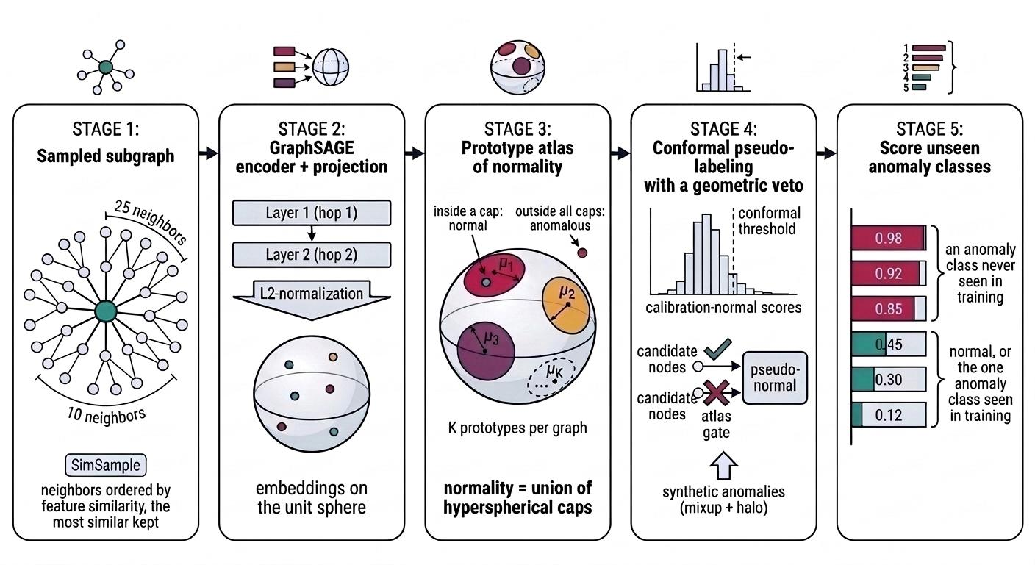
\includegraphics[width=\linewidth]{figures/method_overview.pdf}
\caption{OUTPOST scores a node by how far its embedding falls outside a learned atlas of normality: a 2-layer GraphSAGE encoder over neighbor-sampled subgraphs (fan-out 25 then 10) is projected and $L_2$-normalized onto the unit sphere, where 3 or 8 prototypes with fitted radii define normality as a union of hyperspherical caps, and conformal pseudo-labeling -- vetoed by the atlas for any candidate lying outside every cap -- expands the training signal toward anomaly classes never labeled. Scores shown in stage 5 are illustrative; every measured number in this paper is in the figures and tables that follow.}
\label{fig:method}
\end{figure}

% -------------------------------------------------------------------------
% figure      : figures/selection_noise.pdf
% drawn by    : analysis/scripts/make_figures_paper.py
% result file : analysis/tables/selection_noise.json
% supports    : METHODOLOGY 4.9 -- P35, P40
% -------------------------------------------------------------------------
\begin{figure}[t]
\centering
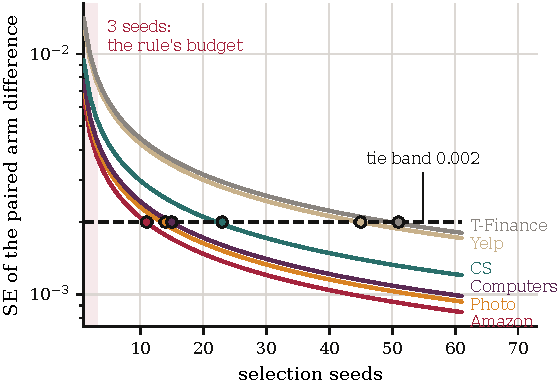
\includegraphics[width=\linewidth]{figures/selection_noise.pdf}
\caption{The 0.002 AUC-ROC tie band used to call two arms equivalent sits below the standard error of a 3-seed comparison on all 6 graphs, and resolving a difference that small would take up to 51 seeds (T-Finance); every tie this paper reports is therefore a statement about noise, not about the methods.}
\label{fig:selection-noise}
\end{figure}

% -------------------------------------------------------------------------
% figure      : figures/oracle_inflation_separation.pdf
% drawn by    : analysis/scripts/make_figures_paper.py
% result file : analysis/tables/inflation_ordering.json
% supports    : METHODOLOGY 3.2
% -------------------------------------------------------------------------
\begin{figure}[t]
\centering
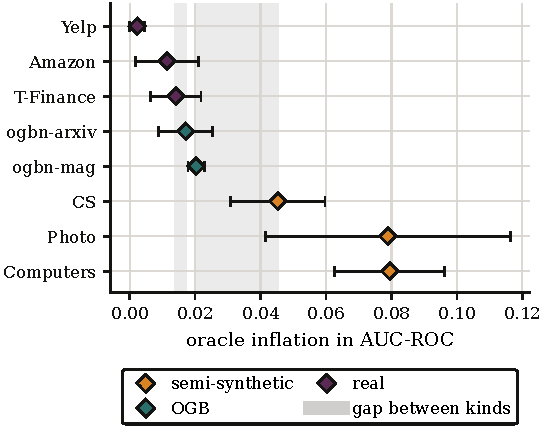
\includegraphics[width=\linewidth]{figures/oracle_inflation_separation.pdf}
\caption{Oracle selection inflates AUC-ROC in strict order of how a benchmark was built -- semi-synthetic above OGB above real, with no overlap between the 8 dataset means (shaded: OGB to semi-synthetic is 0.025 wide, though the closest boundary, real to OGB, is only 0.003 and well inside the run-to-run spread the bars show) -- so best-epoch reporting rewards a method most exactly where the anomalies were manufactured.}
\label{fig:inflation}
\end{figure}

% -------------------------------------------------------------------------
% figure      : figures/mechanism_real_vs_synthetic.pdf
% drawn by    : analysis/scripts/make_figures_paper.py
% result file : analysis/appendix.json (ablations)
% supports    : METHODOLOGY 5.4 -- P28, P39
% -------------------------------------------------------------------------
\begin{figure}[t]
\centering
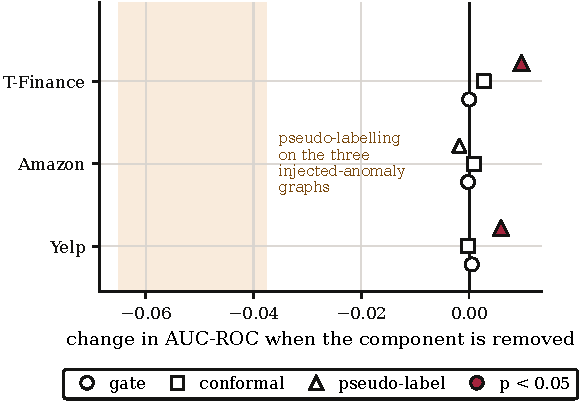
\includegraphics[width=\linewidth]{figures/mechanism_real_vs_synthetic.pdf}
\caption{Removing any of OUTPOST's three components moves AUC-ROC by at most 0.0097 on the 3 graphs whose anomalies were observed rather than injected, while removing pseudo-labeling costs 0.038 to 0.065 on the injected-anomaly graphs (shaded): the mechanism the method is built around is a property of the injection, not of anomaly detection.}
\label{fig:mechanism}
\end{figure}

% -------------------------------------------------------------------------
% figure      : figures/law_crossval.pdf
% drawn by    : analysis/scripts/make_figures_paper.py
% result file : analysis/tables/law_crossval.json
% supports    : METHODOLOGY 6.5
% -------------------------------------------------------------------------
\begin{figure}[t]
\centering
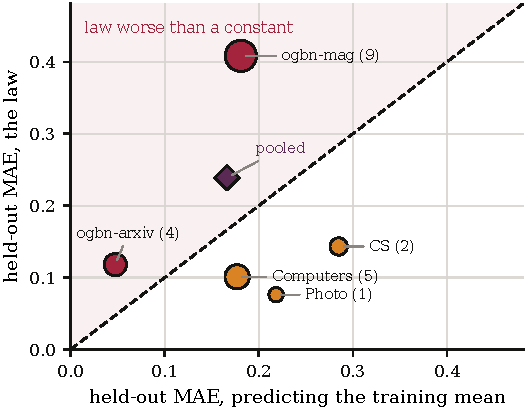
\includegraphics[width=\linewidth]{figures/law_crossval.pdf}
\caption{Held out one dataset at a time, the detectability law's same-class-fraction line predicts the AUC of unseen classes worse than a constant that ignores the diagnostic entirely (pooled MAE 0.239 against 0.166 over 21 classes, the line winning 3 of 5 folds yet losing on pooled error because it fails worst on the largest fold, ogbn-mag at 0.408 against 0.181 on 9 of 21 classes), so the law describes the classes it was fitted on and carries no out-of-sample content.}
\label{fig:law-crossval}
\end{figure}

% -------------------------------------------------------------------------
% figure      : figures/p8_diagnostic_vs_trained.pdf
% drawn by    : analysis/scripts/make_figures_paper.py
% result file : analysis/tables/p8_per_class.json
%               analysis/tables/spectral_ogbn-mag.csv
% supports    : METHODOLOGY 6.6 -- P8
% -------------------------------------------------------------------------
\begin{figure}[t]
\centering
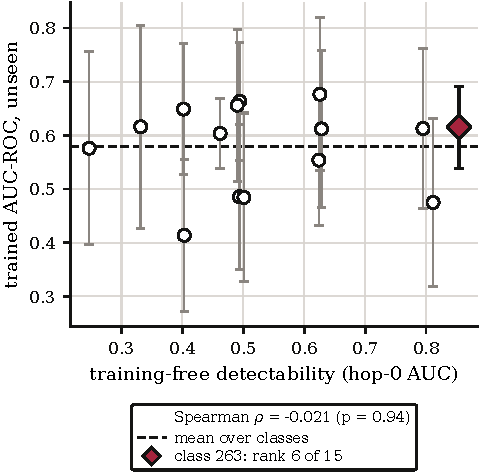
\includegraphics[width=\linewidth]{figures/p8_diagnostic_vs_trained.pdf}
\caption{Across 15 ogbn-mag classes the training-free detectability diagnostic has no rank correlation with what a trained model achieves on the same class unseen ($\rho = -0.021$, $p = 0.94$), and the class the diagnostic rates most detectable ranks 6 of 15 once trained: the diagnostic is not a ceiling.}
\label{fig:p8}
\end{figure}

% -------------------------------------------------------------------------
% figure      : figures/detectability_law.pdf
% drawn by    : analysis/scripts/make_figures_paper.py
% result file : analysis/tables/spectral_*.csv
%               analysis/tables/detectability_law.json
% supports    : METHODOLOGY 6.1-6.2
% -------------------------------------------------------------------------
\begin{figure}[t]
\centering
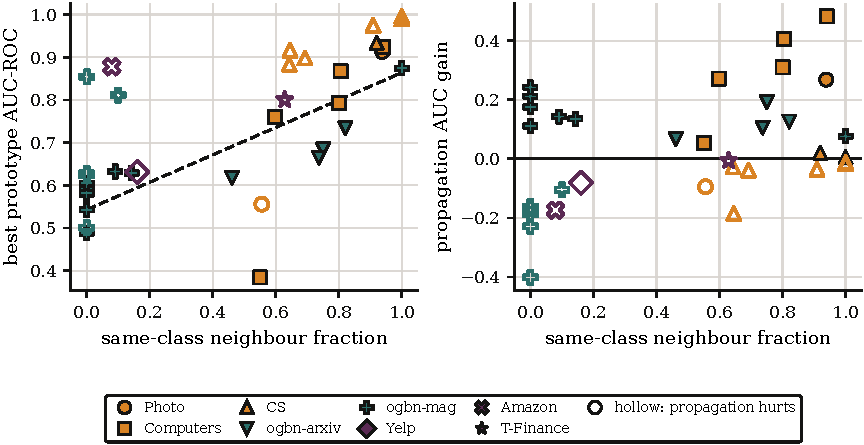
\includegraphics[width=\linewidth]{figures/detectability_law.pdf}
\caption{Across 37 anomaly classes on 8 graphs a class's training-free detectability tracks how clustered it is ($\rho$ = 0.778, permutation $p$ = 5e-05, cluster-bootstrap 95\% CI [0.39, 0.91]), and the right panel says why: propagation amplifies clustered anomalies and erases scattered ones (21 classes in the propagation regime). This describes the classes it was measured on; Figure~\ref{fig:law-crossval} shows it does not predict held-out ones.}
\label{fig:law}
\end{figure}

% -------------------------------------------------------------------------
% figure      : figures/regime_decomposition.pdf
% drawn by    : analysis/scripts/make_figures_paper.py
% result file : analysis/tables/simsample_by_dataset.json
% supports    : METHODOLOGY 5.5 -- P14, P17
% -------------------------------------------------------------------------
\begin{figure}[t]
\centering
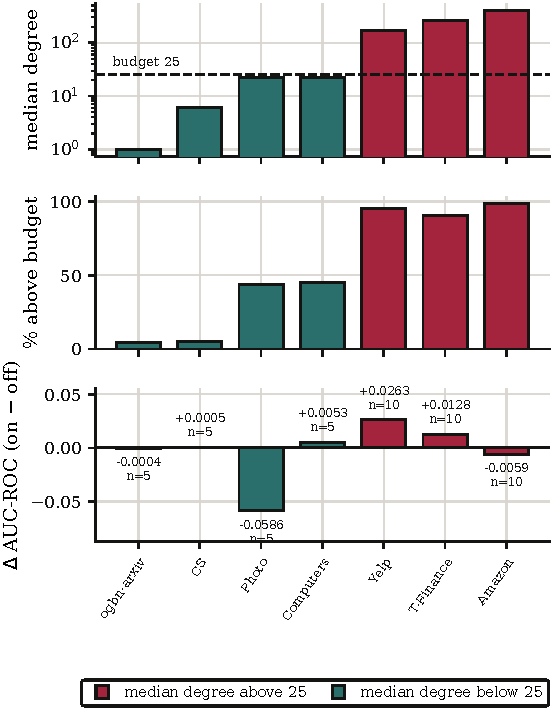
\includegraphics[width=0.62\linewidth]{figures/regime_decomposition.pdf}
\caption{If SimSample worked by restoring neighbors lost to the hop-1 budget of 25, its effect would follow the top two panels; it does not -- of the 3 graphs above the budget 2 improve and 1 does not, and 2 of the 4 graphs below it improve anyway, which falsifies the pre-registered mechanism (P14, P17).}
\label{fig:regime}
\end{figure}

% -------------------------------------------------------------------------
% figure      : figures/simsample_mechanism.pdf
% drawn by    : analysis/scripts/make_figures_paper.py
% result file : results/results.csv (yelp arms)
% supports    : METHODOLOGY 5.5 -- P14, P17
% -------------------------------------------------------------------------
\begin{figure}[t]
\centering
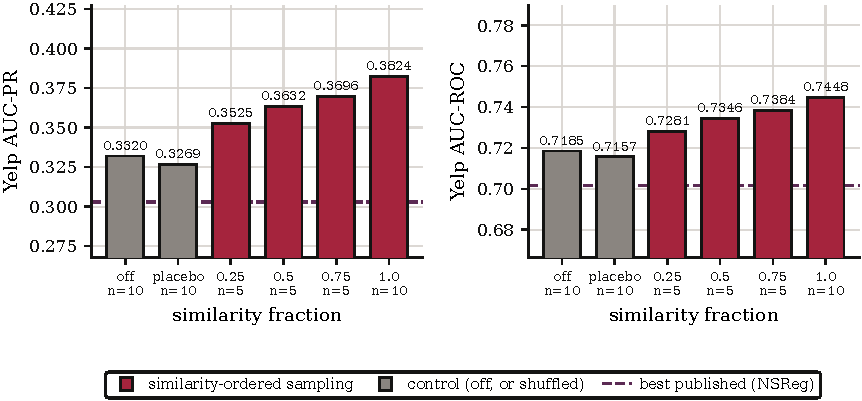
\includegraphics[width=\linewidth]{figures/simsample_mechanism.pdf}
\caption{Shuffling the similarity order while keeping everything else fixed destroys the whole +0.0504 Yelp AUC-PR gain that SimSample gives (0.3824 on): the shuffled placebo lands at 0.3269, below the 0.3320 of turning SimSample off altogether, so the gain comes from the order itself and not from sampling fewer neighbors.}
\label{fig:simsample}
\end{figure}

% -------------------------------------------------------------------------
% figure      : figures/yelp_comparison.pdf
% drawn by    : analysis/scripts/make_figures_paper.py
% result file : analysis/tables/published_baselines.csv
%               results/results.csv
% supports    : METHODOLOGY 5.5
% -------------------------------------------------------------------------
\begin{figure}[t]
\centering
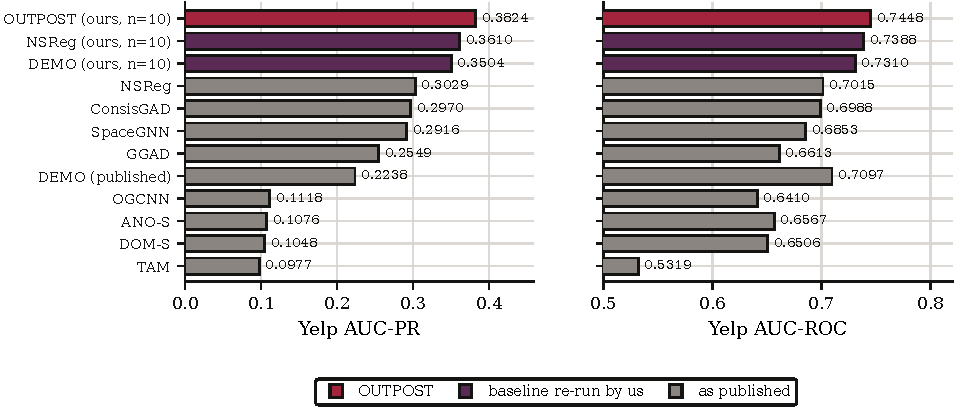
\includegraphics[width=\linewidth]{figures/yelp_comparison.pdf}
\caption{On the one graph in this study whose anomalies are real fraud, OUTPOST reaches 0.3824 AUC-PR against the best published 0.3029 (NSReg), but the same baseline re-run by us under this protocol reaches 0.3610, so most of the apparent margin over the literature is protocol, not method.}
\label{fig:yelp}
\end{figure}

% -------------------------------------------------------------------------
% figure      : figures/efficiency.pdf
% drawn by    : analysis/scripts/make_figures_paper.py
% result file : results/results.csv
%               analysis/tables/published_baselines.csv
% supports    : METHODOLOGY 5.5
% -------------------------------------------------------------------------
\begin{figure}[t]
\centering
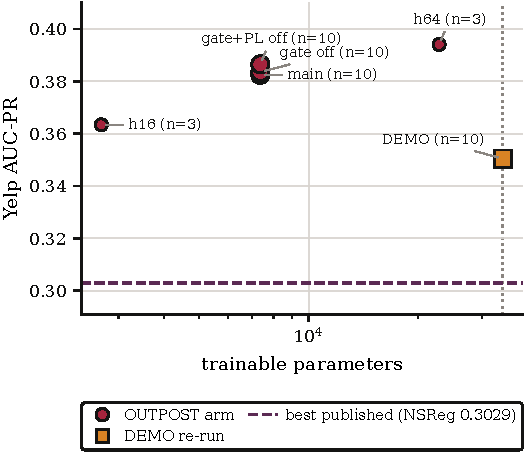
\includegraphics[width=\linewidth]{figures/efficiency.pdf}
\caption{On Yelp, OUTPOST reaches 0.3824 AUC-PR with 7,361 trainable parameters, 0.22$\times$ DEMO's 34,209 and +0.0795 above the best published result (NSReg 0.3029); the two arms that vary width rest on 3 seeds each, which is why they are drawn smaller.}
\label{fig:efficiency}
\end{figure}

